%! Author = Saeid Yazdani
%! Date = 7/14/2024


\section{\acs{PWM} Control for Switching Power Supplies}
\label{sec:pwm-for-switching-supplies}

Since the introduction of solid-state electronics during the 1960s and
1970s, \ac{PWM} have been utilized in power systems to conserve energy.
It was initially used in motor control applications due to its efficiency in
regulating power as the ability to control the duty cycle of a signal allows
for precise regulation of voltage and current, making it ideal for switching
power supplies widely used in applications such as portable electronics
and battery chargers \autocite{6647256}.

\subsection{Basic \acs{PWM} Switching Supply}
\label{subsec:basic-pwm-psu}

A \ac{PWM}-controlled switching power supply converts an input voltage
into a regulated \ac{DC} output by rapidly turning a switch on and off.
The duration of these on/off cycles is controlled by a PWM signal, which adjusts
the average power delivered to the load.

The pulsed output is then smoothed out by an inductive-capacitive filter to
create a smooth \ac{DC} voltage as
shown in \autoref{fig:basic-pwm-supply-concept}.
This filtered \ac{DC} voltage is then supplied to the device and is calculated
according to \autoref{eq:basic-pwm-output-voltage}.

\begin{figure}[htbp]
    \centering
    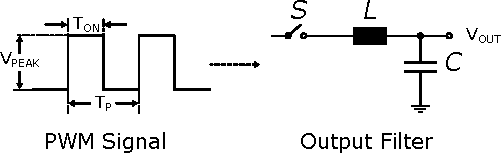
\includegraphics[width=\linewidth,height=0.62\textheight,keepaspectratio]
    {figures/dps_algorithms_psu/basic_pwm_psu_concept}
    \caption[Basic \acs{PWM}-Based \acs{PSU} Concept]{
        Basic concept behind a \ac{PWM} controlled switching power supply is
        based on applying a series of pulses to an
        \emph{Inductive-Capacitive} filter.
    }
    \label{fig:basic-pwm-supply-concept}
\end{figure}

\begin{equation}
    \label{eq:basic-pwm-output-voltage}
    V_{OUT} = \frac{T_{ON}}{T_{P}} \times V_{PEAK}
\end{equation}

\subsection{Challenges With Basic \acs{PWM} Control Schemes}
\label{subsec:challenges-withbasic-pwm-control-schemes}

A major drawback of pure \ac{PWM}-controlled power supplies is that they require
crossing a switching threshold:

\begin{itemize}[topsep=8pt,itemsep=4pt,partopsep=4pt, parsep=4pt]
    \item
    When the output exceeds the target value, the system switches off.

    \item
    When the output falls below the target value, the system switches on.
\end{itemize}

Therefore, the resulting hysteresis band is very narrow and has a limited
dynamic response for fast load changes, adversely affecting the
\emph{transient response} performance in applications where rapid or sudden
changes in load condition are expected
\autocite{paper:fangrui,paper:ngai-man}.

As shown in \autoref{fig:example-transient-response}, transient response of
a power supply is defined as its ability to react to a sudden change in load
conditions with the following aspects:

\begin{itemize}[topsep=8pt,itemsep=4pt,partopsep=4pt, parsep=4pt]
    \item \textbf{Speed of Response:}
    How fast the power supply adjusts its output voltage in response to
    load variations.

    \item \textbf{Overshoot and Undershoot:}
    When the load varies, the output of the power supply can exceed or
    drop below the set target voltage before stabilizing again.

    \item \textbf{Settling Time:}
    The time needed for the output voltage to settle at the set target
    voltage.

    \item \textbf{Stability:}
    The ability to remain stable with minimal oscillations during and after
    transient periods.

\end{itemize}

\begin{figure}[htbp]
    \centering
    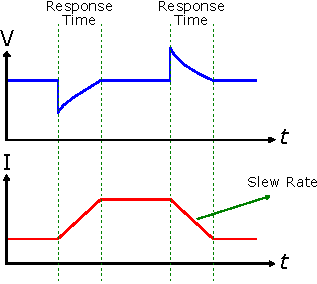
\includegraphics[width=0.64\linewidth,height=0.37\textheight,keepaspectratio]
    {figures/dps_algorithms_psu/response-time-example}
    \caption[Example of Transient Response Time]{
        Transient response deviation and time indicate how the output voltage
        reacts to sudden current changes, including peak deviation and recovery
        time to nominal voltage.
    }
    \label{fig:example-transient-response}
\end{figure}

Measurements and diagnosis presented in \autoref{sec:dps-measurements} and
\autoref{sec:capacitive-load-effects} are mainly indicative for problems
related to transient response as measured by \ac{VDUT} in
\autoref{fig:vdut-result-1v3-10uF} and
\autoref{fig:vdut-result-1v3-4R7}.

One approach to improve transient response is using a linear regulator, which
provides quick voltage adjustments.
However, this method reduces efficiency and is impractical in applications with
high current demand.

Switching regulators with conventional PWM control are more efficient than
linear regulators but have slower transient responses and therefore requiring
large capacitance at the load side \autocite{792807}.
Using more capacitance with low \ac{ESR} is expensive and requires more volume
and board space and has its own drawbacks as discussed in
\autoref{sec:capacitive-load-effects}.

\subsection{Disadvantages of Complex Filter Stages}

With conventional PWM control schemes, hysteresis must be filtered to get smooth
signal waveforms, hence, requiring complex filters on the output side:
The better the output signal quality must be, the higher the filter effort.
This is not a problem if the load can tolerate noise and ripple as is true for
many applications where the load itself is filtering due to their
inductive nature, such as in motor coils.

In an \ac{ATE} environment, test engineers are dealing with \acp{DUT} where
there is no integrated power filtering inside the DUT, so additional digital and
analog filters must be provided by the \ac{ATE} itself.

Complex filter stages are used to reduce noise and ripple, but they come with
major drawbacks:

\begin{itemize}[topsep=8pt,itemsep=4pt,partopsep=4pt, parsep=4pt]
    \item \textbf{Slow Transient Response:}
    Complex filters introduce delay in the transient response as the filters
    delay time-to-stability of the output.

    \item \textbf{Inflexibility:}
    Every \ac{DUT} has its own load characteristic.
    A \ac{DPS} should be flexible for various kinds of \acp{DUT} and
    needs filter stages to cover all kinds of \acp{DUT}, which is impractical.

    \item \textbf{Reduced Efficiency:}
    Filters stages require multiple passive and active components and
    each additional component introduces loss (e.g. core losses and heat
    dissipation in passive components, etc.).

\end{itemize}

Other disadvantages of complex filter stages include \emph{production cost},
\emph{larger size} and \emph{increased power consumption} which may not be of
high concern for an \ac{ATE} in contrast to a mass-produced consumer-grade
system.

